% Тут используется класс, установленный на сервере Papeeria. На случай, если
% текст понадобится редактировать где-то в другом месте, рядом лежит файл matmex-diploma-custom.cls
% который в момент своего создания был идентичен классу, установленному на сервере.
% Для того, чтобы им воспользоваться, замените matmex-diploma на matmex-diploma-custom
% Если вы работаете исключительно в Papeeria то мы настоятельно рекомендуем пользоваться
% классом matmex-diploma, поскольку он будет автоматически обновляться по мере внесения корректив
%
\documentclass[14pt]{matmex-diploma}
\renewcommand{\baselinestretch}{1.5}
\usepackage{float}
\usepackage{hyperref}
\usepackage{minted}
\usepackage{caption}
\usepackage{comment}
\begin{document}
% Год, город, название университета и факультета предопределены,
% но можно и поменять.
% Если англоязычная титульная страница не нужна, то ее можно просто удалить.
\filltitle{ru}{
   chair              = {Кафедра системного программирования},
   title              = {Сравнение алгоритмов табличного восходящего синтаксического анализа},
   type               = {diploma},
   position           = {студента},
   group              = 544,
   author             = {Мавчун Екатерина Валерьевна},
   supervisorPosition = {магистр информационных технологий, ст.преп.},
   supervisor         = {Григорьев С.В.},
   reviewerPosition   = {программист ООО <<ИнтеллиДжей Лабс>>},
   reviewer           = {Подкопаев А.В.},
   chairHeadPosition  = {д.\,ф.-м.\,н., профессор},
   chairHead          = {Терехов А.Н.},
   university         = {Правительство Российской Федерации \\ \bigskip
   Федеральное государственное бюджетное образовательное учреждение высшего профессионального образования \\ \bigskip
   «Санкт-Петербургский государственный университет» \\ \bigskip \\ \bigskip \\ \bigskip},
  faculty            = {}, % Оставить пустым!!!
}
\filltitle{en}{
   type               = {diploma},
   chair              = {Chair of Software Engineering},
   title              = {Comparison of table-based bottom-up parsers},
   author             = {Ekaterina Mavchun},
   supervisorPosition = {master of Information Technology, senior lecturer},
   supervisor         = {Semyon Grigoriev},
   reviewerPosition   = {software developer at <<IntelliJ Labs>>},
   reviewer           = {Anton Podkopaev},
   chairHeadPosition  = {professor},
   chairHead          = {Andrey Terekhov},
   university         = {SAINT-PETERSBURG STATE UNIVERSITY},
   faculty            = {}, % Оставить пустым!!!
   city               = {Saint-Petersburg},
}
\maketitle
\tableofcontents
% У введения нет номера главы
\section*{Введение}
Синтаксический анализатор (парсер) ~--- это программа, которая проверяет текст на соответствие некоторой грамматике и по линейной последовательности токенов этого текста строит дерево разбора (синтаксическое дерево) \cite{book:theory_of_parsing}, которое хорошо подходит для дальнейшей обработки и анализа текста. Синтаксические анализаторы широко используются, например, для создания компиляторов, также они используются в лингвистике, для машинного перевода. Поэтому создание синтаксических анализаторов является важной задачей.
% * <Семён Григорьев> 08:38:34 06 Jun 2015 UTC+0300:
% Распознаёт -- плохой термин в данном контексте. Либо проверяет на соответствие и строит дерево, либо всё предложение перестроить.
% ^ <Ekaterina Mavchun> 15:39:11 06 Jun 2015 UTC+0300:
% Исправила

Существует множество различных типов алгоритмов синтаксического анализа, одним из которых является \textit{восходящий анализ} (bottom-up analysis) \cite{book:grune}, который поддерживает LR(k)-грамматики \cite{book:compilles}, рассматривая цепочки токенов слева направо, и строит правый вывод. При этом узлы синтаксического дерева строятся от листьев (терминальных символов) к корню (начальному символу грамматики). Одним из подходов к реализации восходящего синтаксического анализатора является табличный способ: для грамматики строятся таблица действий и таблица переходов. Первая позволяет задавать следующую операцию анализатора в зависимости от входного терминального символа и текущего состояния анализатора. А вторая определяет состояние в зависимости от нетерминального символа и текущего состояния.

Так как создавать анализаторы вручную достаточно трудоёмко, то разработаны и используются специальные генераторы анализаторов, например, Yacc \cite{link:yacc}, Bison \cite{link:bison}, ANTLR \cite{link:antlr}. Известно \cite{book:compilers_dotNET}, что для любой контекстно-свободной грамматики можно построить анализатор, сложность которого не превышает O($n^3$), где n ~--- это длина входного текста. Но анализаторы реально используемых языков программирования обычно имеют линейную сложность, то есть для заданного языка существует такая грамматика, которая позволяет создать более быстрый анализатор.

В книге \cite{book:grune} доказывается, что известные алгоритмы табличного восходящего анализа ~--- LR(0), LR(1), SLR(1), LALR(1) ~--- имеют линейную сложность. Однако востребовано практическое исследование производительности данных алгоритмов, так как на практике серьёзную роль играют различные константы. То есть на практике производительность анализаторов, соответствующих вышеперечисленным алгоритмам, может оказаться различной. Таким образом, практические и теоретические результаты могут отличаться. Следовательно, для перечисленного набора алгоритмов необходимо на одинаковых входных данных исследовать их производительность. Теоретические сравнительные исследования, в основном, подкрепляются «искусственными» примерами, поэтому важно провести сравнения на более реалистичных грамматиках. При этом целесообразно иметь единую платформу для экспериментов с тем, чтобы иметь возможность запускать различные анализаторы, реализующие соответствующие алгоритмы, и сравнивать время работы на фиксированных входных данных.

На кафедре системного программирования был разработан инструмент для создания синтаксических анализаторов и обработки грамматик YaccConstrutor (YC) \cite{link:yc}. В этом инструменте созданы различные генераторы для создания синтаксических анализаторов: RNGLR, FsYacc и др. \cite{link:yc}. Также существует сторонний инструмент для создания синтаксических и лексических анализаторов ~--- Facio \cite{link:facio}, который поддерживает ряд таких алгоритмов восходящего синтаксического анализа, как LR(0), LR(1), SLR(1), LALR(1). Выбор именно этого инструмента обусловлен тем, что он разработан на платформе .NET \cite{link:dotNet}, язык программирования F\# аналогично инструменту YC. Также Facio содержит необходимые алгоритмы синтаксического анализа. Таким образом, требуется получить унифицированный инструмент, позволяющий работать с алгоритмами обоих инструментов. 

В качестве основы единой платформы, предлагается использовать два инструмента — YC и Facio. Таким образом, чтобы получить единую среду с различными алгоритмами, возникает задача интеграции этих инструментов. Такая платформа может быть использована в учебных целях для изучения и наглядного сравнения различных алгоритмов восходящего синтаксического анализа. Также добавление алгоритмов в YC позволит без лишних усилий создавать необходимые для других задач анализаторы.

\section{Постановка задачи}
Целью данной работы является сравнение производительности различных алгоритмов табличного восходящего синтаксического анализа, поскольку теоретические и практические результаты могут отличаться. Известно, что рассматриваемые алгоритмы линейны, но важно исследовать их производительность относительно друг друга. Для достижения этой цели необходимо решить следующие задачи:
\begin{itemize}
\item
реализовать интеграцию YaccConstructor и Facio;
\item
выполнить сравнение алгоритмов табличного восходящего синтаксического анализа, то есть провести замеры времени работы сгенерированных синтаксических анализаторов в зависимости от размеров входного текста.
\end{itemize}

Практическую реализацию данной работы можно использовать в учебных целях: есть единая среда с некоторым набором генераторов, можно на практике сравнивать производительность синтаксических анализаторов, сгенерированных с помощью различных алгоритмов. Такое сравнение является корректным, поскольку используется один интерпретатор ~--- программа, производящая пооператорный анализ, обработку и выполнение исходной программы.

К тому же инструмент YC активно развивается и используется при решении различных задач, поэтому добавление новых генераторов в YC необходимо, например, для анализа встроенных языков (абстрактного анализа) \cite{abstract_parsing}.

\section{Обзор}
\subsection{Восходящий синтаксический анализ}
Восходящие алгоритмы синтаксического анализа строят синтаксическое дерево снизу вверх, то есть от листьев (терминальных символов) к корню (начальному символу грамматики). При этом исходная цепочка <<сворачивается>> к аксиоме грамматики: подстрока входной цепочки сопоставляется с правой частью правила грамматики, которое заменяется соответствующим этому правилу нетерминалом, то есть левой частью правила. Так как восходящие анализаторы способны анализировать большое количество разнообразных грамматик, то они используются довольно часто, поэтому для данных алгоритмов созданы генераторы ~--- программы, создающие анализаторы.

\subsection{LR(k)-анализаторы}
Восходящий синтаксический анализ позволяет рассматривать LR(k)-грамматики. Рассмотрим аббревиатуру LR(k) более детально:
\begin{itemize}
\item
L обозначает, что входная цепочка просматривается слева направо (Left-to-right scan);
\item
R обозначает, что строится правый вывод цепочки (Rightmost derivation);
\item
не более k символов используется для принятия решения на каждом шаге.
\end{itemize}

При LR(k)-анализе применяется метод <<перенос>>-<<свёртка>> (shift-reduce) с использованием стекового автомата \cite{book:grune}. Идея метода заключается в том, что символы входной цепочки переносятся в стек до тех пор, пока на вершине стека не накопится цепочка, совпадающая с правой частью какого-либо из правил (операция <<перенос>>). Далее все символы этой цепочки извлекаются из стека, и на их место помещается нетерминал, соответствующий этому правилу (операция <<свёртка>>). Входная цепочка допускается автоматом, если после переноса в автомат последнего символа входной цепочки и выполнения операции <<свёртка>> в стеке окажется только аксиома грамматики.

Бывают ситуации, когда при анализе некоторой цепочки анализатор не может решить, делать <<сдвиг>> или <<свёртку>> (конфликт <<сдвиг>> /<<свёртка>>), или не может решить, какую из нескольких <<свёрток>> применить (конфликт <<свёртка>>/<<свёртка>>).

Анализатор состоит из следующих частей: входная цепочка, выход, стек, управляющая программа, таблица действий и таблица переходов. Схема анализатора представлена на рис.~\ref{analysator}.

\begin{figure}[h]
\center{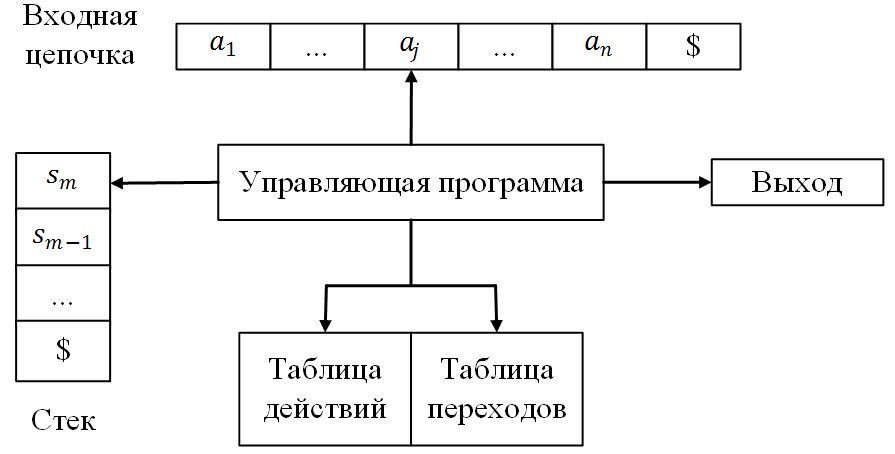
\includegraphics[width=1\textwidth]{Pictures/Analysator.png}}
\caption{Схема анализатора, генерируемого алгоритмом табличного восходящего синтаксического анализа \cite{book:compilers_dotNET}}
\label{analysator}
\end{figure}

Как уже было описано ранее, при выполнении табличного синтаксического анализа для данной грамматики строятся две таблицы: таблица действий и таблица переходов. Таблица переходов ~--- это вспомогательная таблица, используется при одном из действий и может содержать следующие значения:
\begin{itemize}
\item
S ~--- символ состояния;
\item
error ~--- ошибка.
\end{itemize}

Таблица действий определяет дальнейшее действие в текущем состоянии и с текущим символом на входе. Каждый элемент таблицы действий может содержать одно из четырёх значений:
\begin{itemize}
\item
accept (<<успех>>) ~--- разбор входной цепочки завершился успешно;
\item
shift (<<перенос>>) ~--- на вершину стека переносится состояние, которое соответствует входному символу, читается следующий символ;
\item
reduce (<<свёртка>>) ~--- в стеке набрались состояния, которые можно заменить одним, исходя из правил грамматики; значение берётся из таблицы переходов;
\item
error (<<ошибка>>) ~--- анализатор обнаружил ошибку во входной цепочке.
\end{itemize}

\subsection{Алгоритмы, выбранные для исследования}

Восходящим анализаторам соответствуют LR(k)-грамматики. Иерархия подклассов этих грамматик представлена на рис.~\ref{lr_huerarchy}.

\begin{figure}[h]
\center{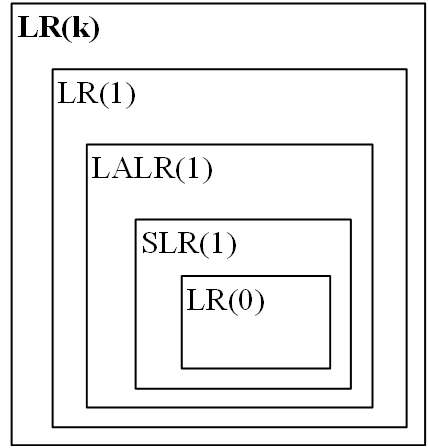
\includegraphics[width=0.4\textwidth]{Pictures/Grammar_types.png}}
\caption{Иерархия подклассов контекстно-свободных грамматик \cite{grammar_type_recognition}}
\label{lr_huerarchy}
\end{figure}

Грамматика является LR(k)-грамматикой, если существует анализатор, написанный для этой грамматики, который читает входные данные слева направо и использует для предпросмотра не более k символов. Эти грамматики могут быть проанализированы восходящими синтаксическими анализаторами.

Для сравнения были выбраны классические, наиболее часто используемые алгоритмы табличного синтаксического восходящего анализа, соответствующие представителям основных подклассов грамматик: LR(0), LR(1), LALR(1), SLR(1). Перечисленные алгоритмы описаны в книге <<Parsing Techniques: A Practical Guide>> \cite{book:grune}. 

Рассмотрим более детально выбранные для исследования алгоритмы табличного восходящего синтаксического анализа.
\begin{enumerate}
\item
\textbf{LR(0)} \\Left-to-right scan Rightmost derivation (0) ~--- генератор синтаксического анализатора для LR(0)-грамматик. Для анализа использует только содержимое стека.
\item
\textbf{LR(1)} \\Left-to-right scan Rightmost derivation (1) ~--- генератор синтаксического анализатора для LR(1)-грамматик. Для принятия решения использует один символ входной цепочки.
\item
\textbf{SLR(1)} \\Simple LR(1) ~--- Simple LR(1). Более мощный алгоритм, чем LR(0), но менее мощный, чем LR(1) и LALR(1). Количество состояний, т.е. строк таблицы, такое же как у LR(0), но данный алгоритм автоматически решает некоторые конфликты.
\item
\textbf{LALR(1)} \\Look-Ahead LR(1) ~--- Look-Ahead LR(1). Упрощённый LR(1)-алгоритм, достаточно мощный для того, чтобы провести синтаксический анализ большинства языков, избегая при этом больших таблиц, в отличие от LR(1)-анализатора. При использовании данного алгоритма можно получить таблицы меньшего размера в результате слияния любых двух состояний, которые совпадают с точностью до символов входной строки, то есть таблицы LALR(1)-анализатора получаются из таблиц LR(1)-анализатора слиянием <<эквивалентных>> состояний в одно. Количество состояний такое же как у LR(0). Данный алгоритм способен решать большее количество конфликтов автоматически, чем SLR(1).
\end{enumerate}

\subsection{Проект YaccConstructor}
% * <Семён Григорьев> 08:46:27 06 Jun 2015 UTC+0300:
% Ни в YC, ни в Facio не сказано, что они на .NET и на F#. Это стоит упомянуть явно в каждом из инструментов, чтобы в интеграции сказать про то, что они на одном языке и на одной платформе и это хорошо.
% ^ <Ekaterina Mavchun> 15:57:52 06 Jun 2015 UTC+0300:
% Дописала в разделы про инструменты и в раздел с интеграцией.
YC \cite{synt_analysis} ~--- это инструмент, который используется для создания синтаксических анализаторов и обработки грамматик, позволяет создавать анализаторы с использованием различных алгоритмов синтаксического анализа, таких как RNGLR, FParsec, FsYacc и др. YC разработан на платформе .NET \cite{link:dotNet}, язык программирования ~--- F\# \cite{link:fSharp}. YC имеет модульную структуру, которая изображена на рис.~\ref{YC}.
Более детальное описание компонент:
\begin{itemize}
\item
\textit{Frontend} ~--- языки задания атрибутной грамматики, которые поддерживает YC, например, Yard, FsYacc, AntLR;
\item
\textit{Intermediate Language} ~--- внутреннее представление анализатора;
\item
\textit{Conversions} ~--- общие преобразования грамматик, например, преобразование, приводящее грамматику к нормальной форме Хомского (CNF); 
\item
\textit{Backend} ~--- при помощи него на основе внутреннего представления генерируется конечный продукт для пользователя. В том числе это и алгоритмы синтаксического анализа: FParsec, FsYacc, RNGLR, YardPrinter, GLL.
\end{itemize}

\begin{figure}[h]
  \center{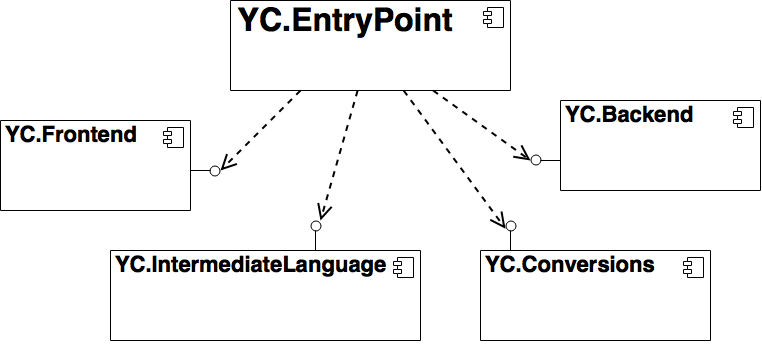
\includegraphics[width=1\textwidth]{Pictures/YC.png}}
  \caption{Архитектура инструмента YC}
  \label{YC}
\end{figure}

Входная грамматика, описанная на одном из поддерживаемых языков описания трансляций, преобразуется во внутреннее представление (IL ~--- Intermediate Language), к внутреннему представлению применяются общие преобразования, и далее по внутреннему представлению конструируется таблица анализатора, соответствующая указанному генератору.

\newpage
\subsection{Проект Facio}
Facio ~--- это инструмент, предназначен для создания лексических и синтаксических анализаторов, включает в себя библиотеку для создания, обработки и анализа контекстно-свободных грамматик. Facio реализован на платформе .NET \cite{link:dotNet}, язык программирования ~--- F\# \cite{link:fSharp}. Структура инструмента Facio изображена на рис.~\ref{Facio}.
Facio состоит из следующих компонент:
\begin{itemize}
\item
\textit{Frontend} ~--- язык задания атрибутной грамматики, например, FsYacc;
\item
\textit{Intermediate Language} ~--- внутреннее представление анализатора;
\item
\textit{Backend} ~--- при помощи него на основе внутреннего представления генерируется конечный продукт для пользователя. В том числе это и алгоритмы синтаксического анализа, такие как LR(0), LR(1), LALR(1), SLR(1).
\end{itemize}

\begin{figure}[h]
  \center{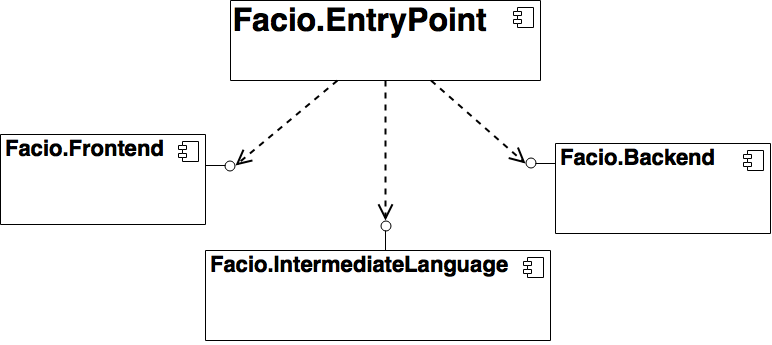
\includegraphics[width=1\textwidth]{Pictures/Facio.png}}
  \caption{Архитектура инструмента Facio}
  \label{Facio}
\end{figure}


\section{Интеграция YaccConstructor с Facio}
Как уже было описано ранее, Facio позволяет конструировать синтаксические анализаторы с использованием различных алгоритмов, которые не реализованы в YC. Чтобы иметь единую среду, поддерживающую алгоритмы, реализованные и в YC и в Facio, необходимо реализовать интеграцию этих инструментов. Как было указано ранее, оба инструмента реализованы на одном языке и на одной платформе.

Структура инструмента, получившегося в результате интеграции, изображена на рис~\ref{YC_after}:
\begin{itemize}
\item
\textit{YC.FacioBackend} ~--- модуль, преобразующий внутреннее представление, оформлен как генератор, который можно указать в аргументах при запуске YC. То есть после того, как входная грамматика была преобразована во внутреннее представление YC, над этим внутренним представлением происходит преобразование форматов, в результате которого получается внутреннее представление Facio. После этого есть возможность использовать любой генератор, реализованный в рамках проекта Facio;
\item
\textit{YC.NoAlt.Conversion} ~--- реализованное общее преобразование грамматик (удаление верхнеуровневых альтернатив);
\item
\textit{Facio} ~--- модуль, соответствующий инструменту Facio (рис.~\ref{Facio}).
\end{itemize}

\begin{figure}[h]
  \center{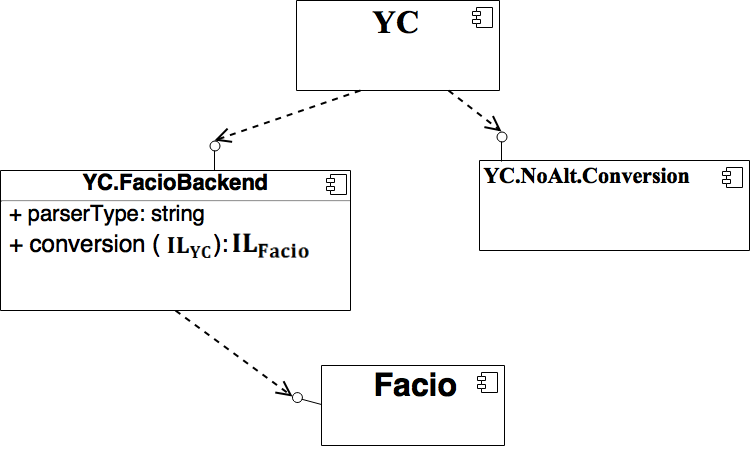
\includegraphics[width=1\textwidth]{Pictures/Integrate_2.png}}
  \caption{Интеграция YC с Facio}
  \label{YC_after}
\end{figure}
\newpage
\subsection{Преобразование внутренних представлений (IL)}
Каждый из инструментов имеет своё внутреннее представление, то есть в каждом инструменте по-разному хранятся данные (терминалы, нетерминалы, правила и т.д.). Таким образом, необходимо реализовать набор преобразований одного внутреннего представления в другое.

Рассмотрим внутреннее представление для каждого из инструментов.
\subsubsection{Внутреннее представление YaccConstructor}
Язык описания трансляций Yard представляет грамматику в виде, описанном на листинге \ref{lst:yardGrammar}.

\begin{listing}[H]
\begin{minted}
[
frame=lines,
framesep=2mm,
baselinestretch=1.2,
fontsize=\small
]
{ruby}
grammar: ('{'header'}')? rules ('{'footer'}')?
\end{minted}
\caption{Грамматика, описанная на Yard}
\label{lst:yardGrammar}
\end{listing}

Здесь: \textit{header} ~--- текст перед описанием грамматики, например, объявление импорта, начинающееся с ключевого слова open; \textit{footer} ~--- текст после описания грамматики; \textit{rules} ~--- правила грамматики.

Входная грамматика преобразуется во внутреннее представление. В YC в роли внутреннего представления анализатора выступает модуль \textit{Definition} (листинг~\ref{lst:YCparser}), который содержит следующие элементы:
\begin{itemize}
\item
\textit{info} ~--- информация (например, происхождение) об этом описании грамматики;
\item
\textit{head} ~--- текст перед описанием грамматики;
\item
\textit{grammar} ~--- само описание грамматики;
\item
\textit{foot} ~--- текст после описания грамматики;
\item
\textit{tokens} ~--- токены с указанием типа;
\item
\textit{'patt} ~--- тип атрибутов (аргументов);
\item
\textit{'expr} ~--- тип выражения в семантическом действии (\textit{action code}).
\end{itemize}

\begin{listing}[H]
\begin{minted}
[
frame=lines,
framesep=2mm,
baselinestretch=1.2,
fontsize=\small
]
{fsharp}
module Definition =     
    type info = { fileName : string }
    type t<'patt,'expr
        when 'patt : comparison and 'expr : comparison> = {
        info    : info;
        head    :'expr option;
        grammar : Grammar.t<'patt,'expr>;
        foot    :'expr option;
        options : Map<string, string>
        tokens  : Map<string, string option>
    }    
\end{minted}
\caption{Внутреннее представление синтаксического анализатора в инструменте YC}
\label{lst:YCparser}
\end{listing}

В свою очередь, \textit{Grammar} (листинг~\ref{lst:YCgrammar}) ~--- это список элементов типа \textit{Module}:
\begin{itemize}
\item
тип \textit{Module} ~--- список правил;
\item
\textit{allPublic} ~--- указывает все ли правила являются публичными, то есть видны из других модулей.
\end{itemize}


\begin{listing}[H]
\begin{minted}
[
frame=lines,
framesep=2mm,
baselinestretch=1.2,
fontsize=\small
]
{fsharp}
module Grammar =  
    type Module<'patt,'expr> = {
        rules     : Rule.t<'patt,'expr> list
        openings  : Source.t list
        name      : Source.t option
        allPublic : bool
    }
    type t<'patt,'expr> = Module<'patt,'expr> list
\end{minted}
\caption{Внутреннее представление грамматики в инструменте YC}
\label{lst:YCgrammar}
\end{listing}

Каждое правило имеет следующую структуру (листинг~\ref{lst:YCrule}):
\begin{itemize}
\item
\textit{name} ~--- имя правила, используется для того, чтобы ссылаться на данное правило из других правил;
\item
\textit{args} ~--- наследуемые аргументы правила;
\item
\textit{body} ~--- тело правила (продукция);
\item
\textit{isStart} ~--- указывает, является ли это правило стартовым, если является, то перед правилом пишется <<[<Start>]>>;
\item
\textit{isPublic} ~--- указывает является ли правило публичным (перед правилом указано <<public>>);
\item
\textit{metaArgs} ~--- список мета-аргументов (имён правил, параметризующих данное правило).
\end{itemize}

\begin{listing}[H]
\begin{minted}
[
frame=lines,
framesep=2mm,
baselinestretch=1.2,
fontsize=\small
]
{fsharp}
module Rule = 
    type t<'patt,'expr> = {
        name     : Source.t
        args     :'patt list
        body     : (Production.t<'patt,'expr>)
        isStart  : bool
        isPublic : bool
        metaArgs :'patt list
    }
\end{minted}
\caption{Внутреннее представление правил в инструменте YC}
\label{lst:YCrule}
\end{listing}

Продукция имеет структуру, указанную в листинге \ref{lst:YCproduction}.
\begin{itemize}
\item
\textit{omit} ~--- указывает, нужно ли включать правило в абстрактное синтаксическое дерево (AST);
\item
\textit{rule} ~--- правило, соответствующее данной продукции;
\item
\textit{binding} ~--- связывание, позволяет писать, например, f:F или f:=F;
\item
\textit{checker} ~--- условие в продукции;
\item
\textit{t} ~--- тип узла продукции в дереве вывода, может принимать следующие значения:
  \begin{itemize}
  \item
  \textit{PAlt} ~--- альтернатива: (e1 | e2);
  \item
  \textit{PSeq} ~--- последовательность атрибутов;
  \item
  \textit{PToken} ~--- токены, конечные элементы синтаксического анализа;
  \item
  \textit{PRef} ~--- ссылка на другой нетерминал внутри продукции (вместе с дополнительным списком аргументов).
  \\Также \textit{t} может принимать значения \textit{PMany}, \textit{PMetaRef}, \textit{PLiteral}, \textit{PRepet}, \textit{PPerm}, \textit{PSome}, \textit{POpt}.
  \end{itemize}
\end{itemize}

\begin{listing}[H]
\begin{minted}
[
frame=lines,
framesep=2mm,
baselinestretch=1.2,
fontsize=\small
]
{fsharp}
module Production = 
    type IRuleType
    type DLabel = {
        label  : string;
        weight : float option
    }
    type elem<'patt,'expr> = {
        omit    : bool;
        rule    : (t<'patt,'expr>);
        binding :'patt option;
        checker :'expr option
    }
    and t<'patt,'expr> = 
        |PAlt     of (t<'patt,'expr>) * (t<'patt,'expr>)
        |PSeq     of (elem<'patt,'expr>) list * 'expr option * DLabel option
        |PToken   of Source.t 
        |PRef     of Source.t * 'expr option
        ...
\end{minted}
\caption{Внутреннее представление продукции в инструменте YC}
\label{lst:YCproduction}
\end{listing}    

\subsubsection{Внутреннее представление Facio}
В инструменте Facio спецификация синтаксического анализатора (листинг~\ref{lst:FacioSpecification}) для грамматики содержит следующие элементы:
\begin{enumerate}
\item
\textit{Header} и \textit{Footer} ~--- текст перед и после описания грамматики соответственно;
\item
\textit{NonterminalDeclarations} ~--- ассоциативный массив для стартовых нетерминалов: ключ ~--- тип нетерминалов, значение ~--- список нетерминалов, имеющих этот тип. \\\textit{StartingProductions} ~--- список стартовых нетерминалов грамматики;
\item
\textit{TerminalDeclarations} ~--- ассоциативный массив: ключ ~--- тип терминалов, значение ~--- список терминалов, имеющих этот тип;
\item
\textit{Associativities} ~--- явное объявление ассоциативности терминалов;
\item
\textit{Productions} ~--- правила, представляющие собой список пар \textit{(нетерминал, список продукций)}, где каждый элемент списка продукций содержит:
  \begin{itemize}
  \item
  символы (список терминалов или нетерминалов, соответствующих текущей продукции);
  \item
  семантическое действие, которое будет выполнено в результате применении данного правила.
  \end{itemize}
\end{enumerate}

\begin{listing}[H]
\begin{minted}
[
frame=lines,
framesep=2mm,
baselinestretch=1.2,
fontsize=\small
]
{fsharp}
type Specification = {
    Header : CodeFragment option;
    Footer : CodeFragment option;
    NonterminalDeclarations : (DeclaredType * NonterminalIdentifier) list;
    TerminalDeclarations : (DeclaredType option * TerminalIdentifier list) list;
    StartingProductions : NonterminalIdentifier list;
    Associativities : (Associativity * TerminalIdentifier list) list;
    Productions : (NonterminalIdentifier * ProductionRule list) list;
}
\end{minted}
\caption{Внутреннее представление синтаксического анализатора в инструменте Facio}
\label{lst:FacioSpecification}
\end{listing}

%==========================================================================
\begin{comment}
Грамматика (листинг~\ref{lst:FacioGrammar}) содержит:
\begin{itemize}
\item
\textit{Terminals} ~--- множество терминалов грамматики;
\item
\textit{Nonterminals} ~--- множество нетерминалов грамматики;
\item
\textit{Productions} ~--- правила грамматики;
\item
\textit{ProductionRuleCount} ~--- кол-во продукций правил, определённых в грамматике;
\item
\textit{Augment} ~--- расширение грамматики начальным символом и маркером конца файла;
\item
\textit{ProductionRuleIds} ~--- добавление идентификатора продукции\\(ключ~--- нетерминал, значение ~--- идентификатор);
\item
\textit{SymbolSets} ~--- возвращает множества, содержащие нетерминалы и терминалы, используемые продукциями грамматики;
\item
\textit{AugmentedGrammar} ~--- расширенная грамматика.
\end{itemize}

\begin{listing}[H]
\begin{minted}
[
frame=lines,
framesep=2mm,
baselinestretch=1.2,
fontsize=\small
]
{fsharp}
type Grammar<'Nonterminal, 'Terminal
    when 'Nonterminal : comparison
    and 'Terminal     : comparison> = {
        Terminals     : Set<'Terminal>;
        Nonterminals  : Set<'Nonterminal>;
        Productions   : Map<'Nonterminal, Symbol<'Nonterminal, 'Terminal>[][]>;
    } with
    member private this.ProductionRuleCount
    static member Augment
    static member ProductionRuleIds
    static member SymbolSets
and AugmentedGrammar<'Nonterminal, 'Terminal>
\end{minted}
\caption{Внутреннее представление грамматики в инструменте Facio}
\label{lst:FacioGrammar}
\end{listing}
\end{comment}
%======================================================================

\subsubsection{Реализация преобразования IL}
В рамках задачи интеграции на стороне YC был добавлен генератор со своим преобразованием, которое позволяет перевести внутреннее представление YC во внутреннее представление Facio.

Рассмотрим основные методы, реализованные в генераторе, позволяющие из внутреннего представления YC получить внутреннее представление Facio:
\begin{enumerate}
\item
Поля \textit{header} и \textit{footer} берутся без изменений.
\item
Получение стартовых нетерминалов осуществляется путём обхода всех правил грамматики и проверки значения поля \textit{isStart}. Далее в качестве типа добавляется символ <<\_>> для автоматического вывода типа.
\item
Множество всех терминалов получается путём обхода всех правил грамматики и сравнения типа продукции с PToken. Также есть функция, возвращающая ассоциативный массив, который сопоставляет каждому используемому типу список терминалов этого типа. Терминалы и их типы извлекаются из поля tokens модуля \textit{Definition}, если для какого-то токена тип не указан, то берётся тип по умолчанию, указанный в аргументах.
\item
Ассоциативность не используется в YC.
\item
Чтобы получить продукции в нужном формате, необходимо обойти все правила грамматики, извлечь информацию об аргументах и семантическом действии.
Аргументы и семантическое действие для правила, берутся из аргументов \textit{PSeq}.
\end{enumerate}


\subsection{Выбор генератора на стороне Facio}
Если используется ранее реализованный в YC генератор, то необходимо просто указать этот генератор в аргументах YC. Для случая, когда используется генератор, реализованный в Facio, добавлен ключ \textit{parserType}. То есть на стороне YC необходимо выбрать генератор, осуществляющий преобразование внутренних представлений, но также необходимо предоставить возможность выбирать генератор на стороне Facio. Ключ \textit{parserType} также указывается в качестве аргумента при запуске YC.

Кроме того добавлен механизм, позволяющий в зависимости от указанного значения ключа \textit{parserType} вызывать соответствующий алгоритм генерации синтаксического анализатора.

\subsection{Добавление преобразования общего вида}
Иногда грамматикам предъявляют некоторые требования, например, из-за особенностей конкретного генератора синтаксических анализаторов. В YC такие требования реализованы в виде ограничений (\textit{Constraints}). Ограничение проверят конкретное свойство грамматики. Также в YC имеются преобразования грамматик общего вида (\textit{Conversions}). Каждому ограничению соответствует некоторое преобразование, позволяющее привести грамматику к нужному виду. Например, есть проверка на то, что грамматика приведена к нормальной форме Хомского.

В ходе работы выяснилось, что ни один из ранее реализованных в YC алгоритмов синтаксического анализа не выдвигал к грамматике требования отсутствия верхнеуровневых альтернатив, поэтому данное преобразование было реализовано.

\section{Эксперименты}
\subsection{Методика проведения эксперимента}
Определим цель эксперимента как сравнение производительности набора алгоритмов табличного восходящего синтаксического анализа, а именно: LR(0), LR(1), SLR(1), LALR(1). Также необходимо выяснить, корректно ли выполнена интеграция инструментов YC и Facio. Следуя \cite{qma} сформируем следующие вопросы, на которые эксперимент должен ответить.
\begin{enumerate}
\item
Сравнить быстродействие исследуемых алгоритмов.
\item
Определить, какой из алгоритмов является самым быстрым / медленным по времени выполнения синтаксического анализа.
\end{enumerate}

Для ответов на эти вопросы была использована следующая метрика: измерение времени работы синтаксических анализаторов, сгенерированных с помощью различных алгоритмов, на одинаковых входных данных.

Параметры компьютера, на котором проводились эксперименты были следующими:
\begin{itemize}
\item
операционная система: Windows 8.1;
\item
процессор: AMD FX(tm)-6100 Six-Core Processor 3.30 GHz;
\item
ОЗУ: 16 ГБ.
\end{itemize}

Все рассматриваемые алгоритмы реализованы на языке программирования F\# \cite{link:fSharp}, то есть выбранные алгоритмы сравниваются в одинаковых условиях.

Схема эксперимента изображена на рис.\ref{Interpreter} и заключается в следующем. Есть грамматика некоторого языка и лексическая спецификация, также есть последовательность входных цепочек разной длины. Для грамматики генерируются синтаксические анализаторы, соответствующие исследуемым алгоритмам. По лексической спецификации генерируется лексический анализатор. Интерпретатор используется один, независимо от выбранного алгоритма, поэтому можно проводить сравнение алгоритмов.

\begin{figure}[h]
  \center{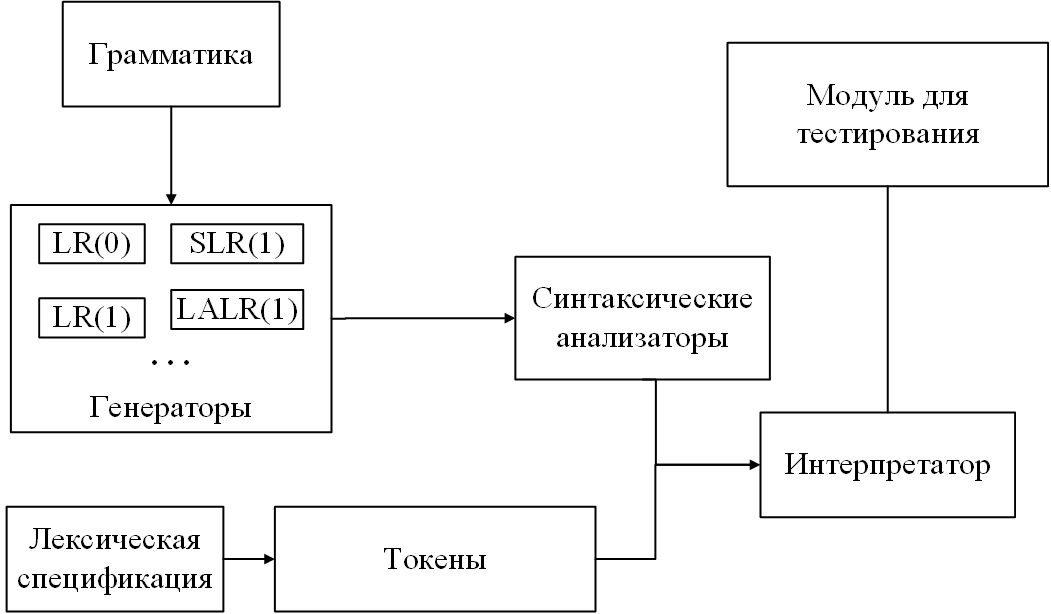
\includegraphics[width=1\textwidth]{Pictures/Interpreter.png}}
  \caption{Схема проведения эксперимента}
  \label{Interpreter}
\end{figure}

После запуска интерпретатора на выходе в модуле для замеров получаем время работы синтаксического анализатора в зависимости от длины входной цепочки. По данным времени работы строится график зависимости времени работы от длины входных данных, и таким образом можно определить, какой из алгоритмов работает быстрее или медленнее.

\subsection{Эксперимент 1}
Проведём сравнение алгоритмов, используя грамматику \textit{EasyCalc}, представленную на листинге~\ref{lst:EasyCalc}.
\begin{listing}[H]
\begin{minted}
[
frame=lines,
framesep=2mm,
baselinestretch=1.2,
fontsize=\small
]
{fsharp}
[<Start>]
s: expr EOF { $1 }
expr : expr MULT numb { $1 * $3 }
     | expr PLUS numb { $1 + $3 }
     | numb { $1 }
numb : ZERO { 0 } | ONE { 1 }
\end{minted}
\caption{Грамматика \textit{EasyCalc}}
\label{lst:EasyCalc}
\end{listing}

{\large \textbf{Результаты сравнения}}

На рис.~\ref{EasyCalcLR0}, \ref{EasyCalcLR1}, \ref{EasyCalcSLR1}, \ref{EasyCalcLALR1} изображена зависимость среднего времени работы синтаксического анализатора по 10-ти запускам от длины входной цепочки для LR(0), LR(1), SLR(1), LALR(1) алгоритмов соответственно. Входная цепочка представляла собой последовательность из <<0>> и <<1>> со знаками <<*>> и <<+>> между ними. Длина входной цепочки изменяется от 2 000 до 10 000 000 токенов.

\begin{figure}[h]
  \center{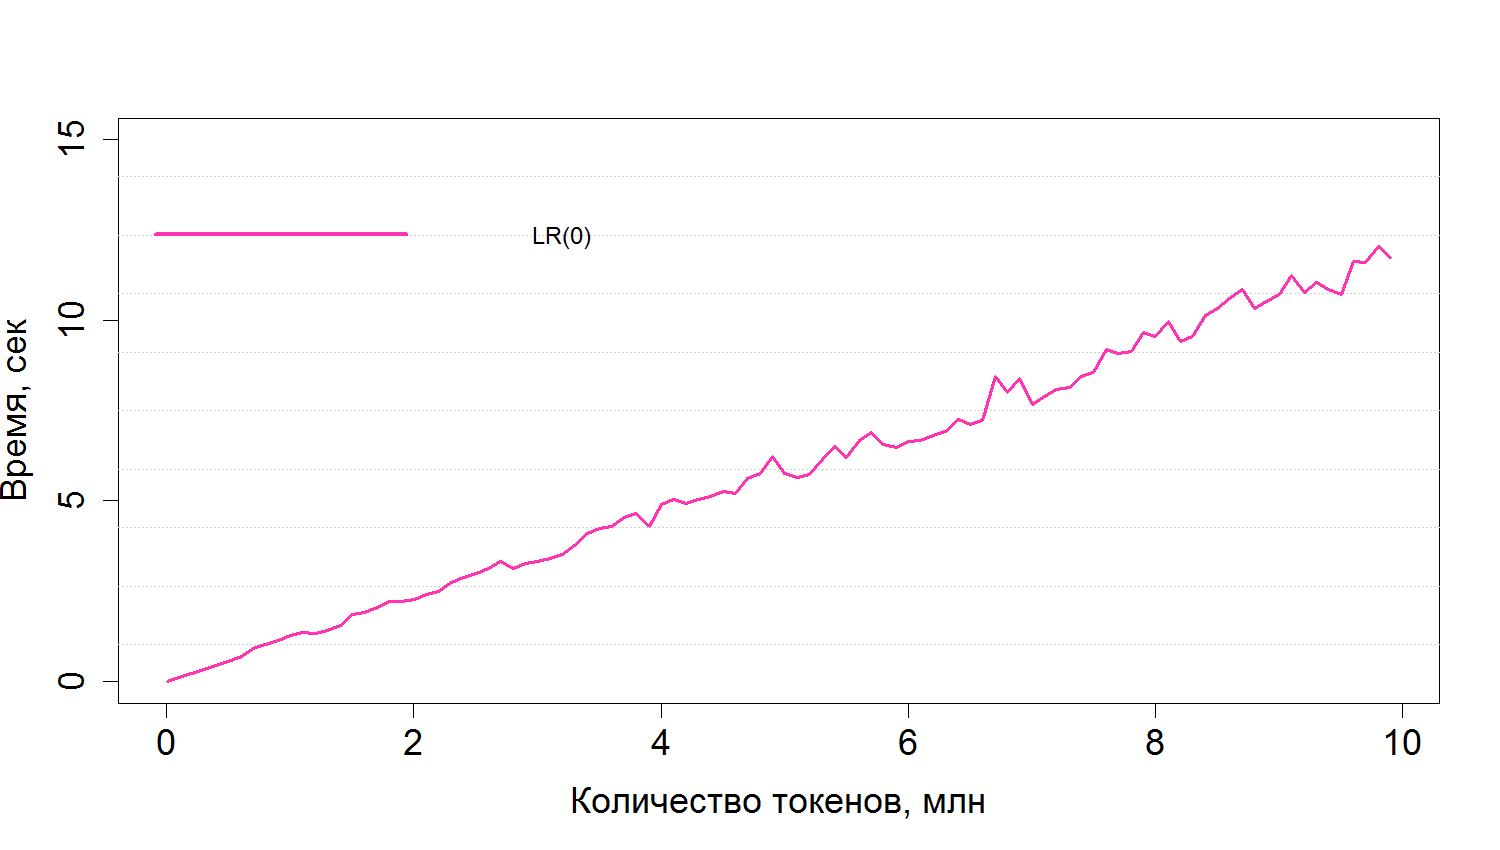
\includegraphics[width=1\textwidth]{EasyCalc/LR0.png}}
  \caption{Время работы LR(0)-анализатора для грамматики \textit{EasyCalc}}
  \label{EasyCalcLR0}
  \centering
\end{figure}


\begin{figure}[H]
  \center{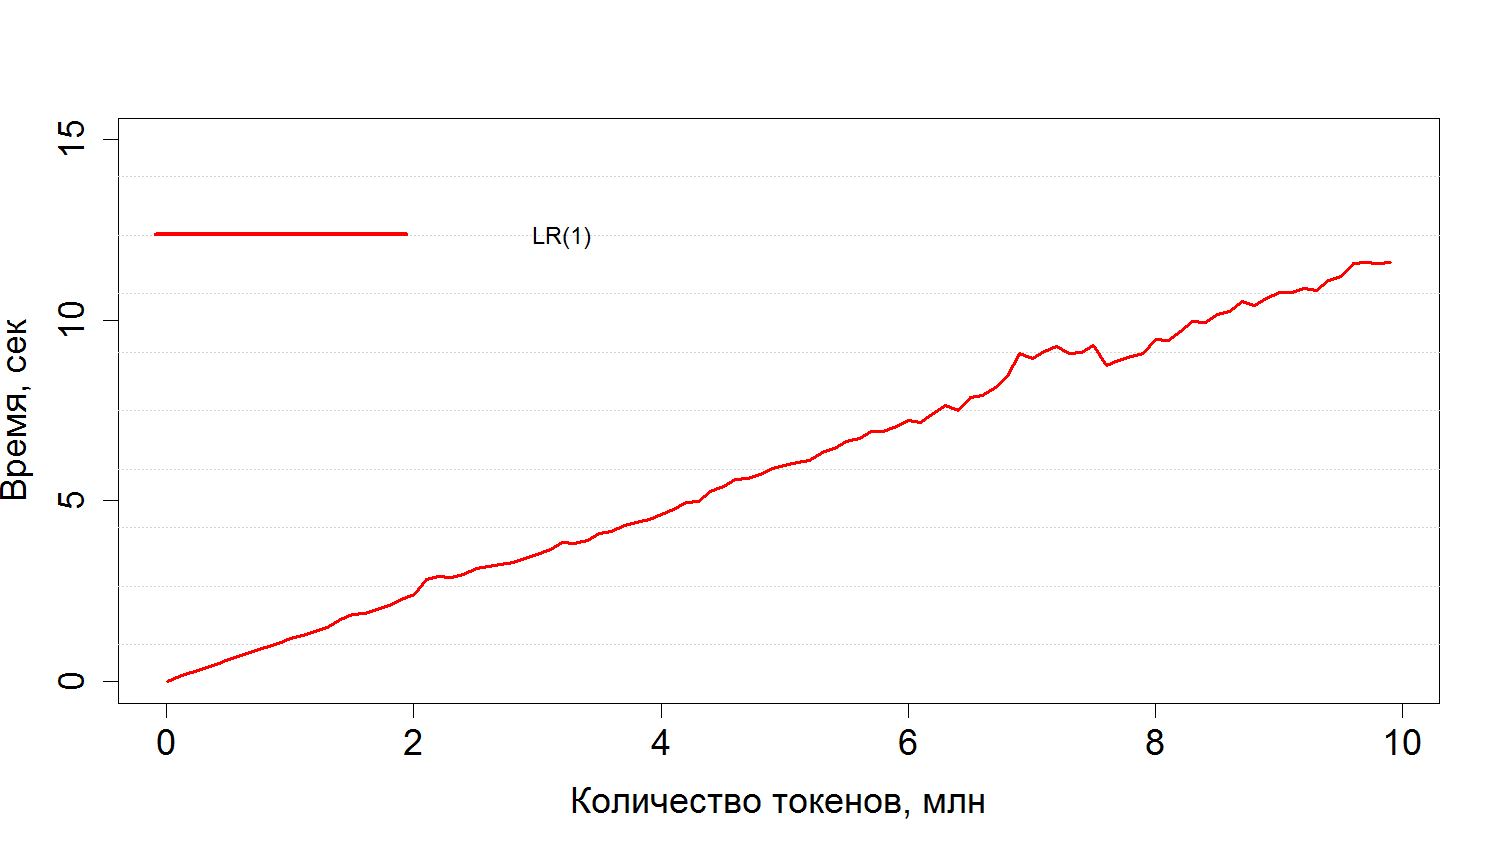
\includegraphics[width=1\textwidth]{EasyCalc/LR1.png}}
  \caption{Время работы LR(1)-анализатора для грамматики \textit{EasyCalc}}
  \label{EasyCalcLR1}
  \centering
\end{figure}


\begin{figure}[h]
  \center{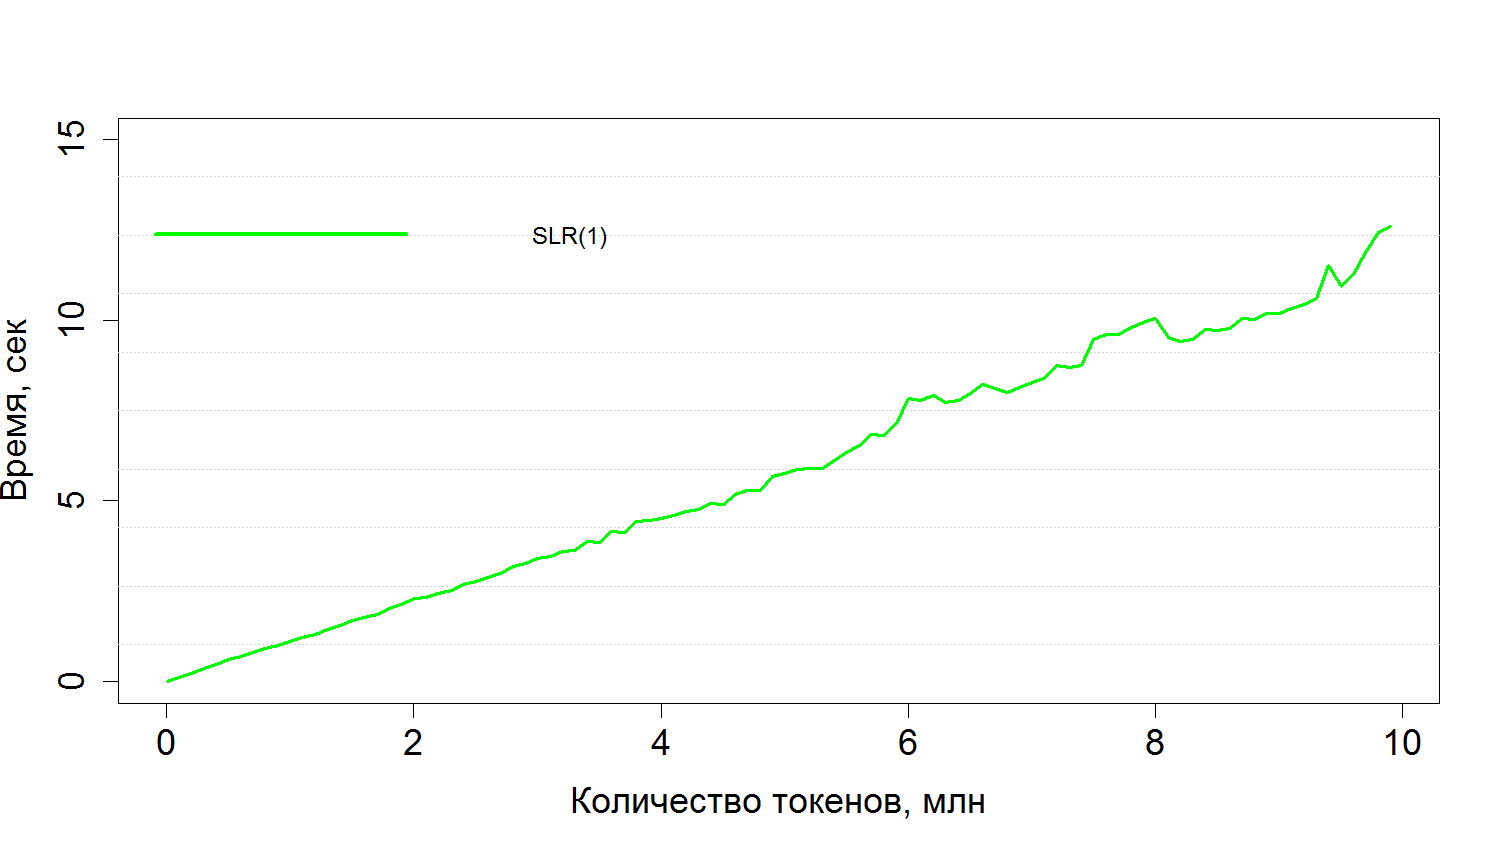
\includegraphics[width=1\textwidth]{EasyCalc/SLR1.png}}
  \caption{Время работы SLR(1)-анализатора для грамматики \textit{EasyCalc}}
  \label{EasyCalcSLR1}
  \centering
\end{figure}


\begin{figure}[H]
  \center{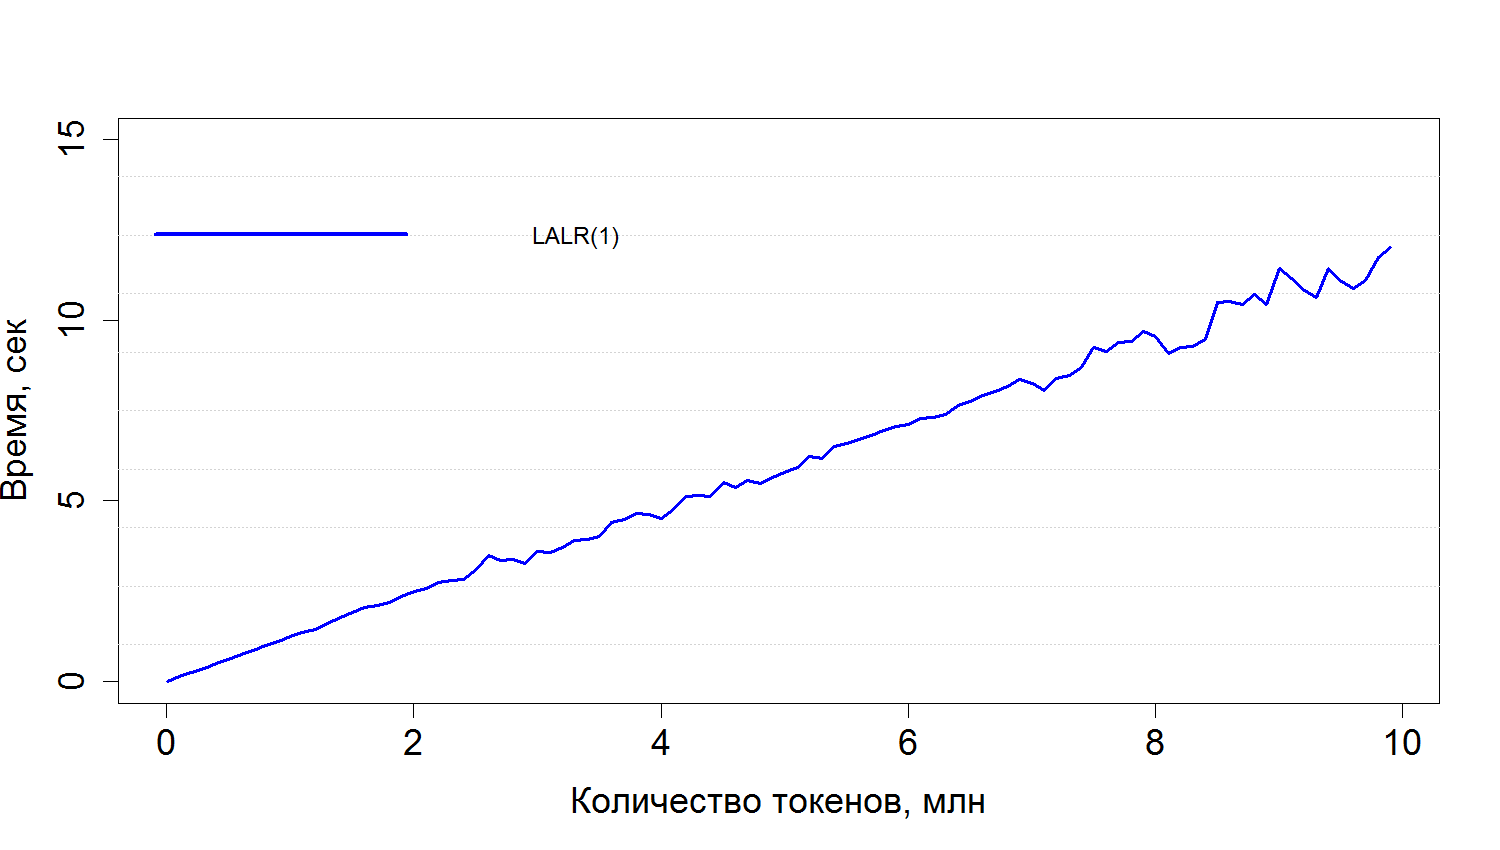
\includegraphics[width=1\textwidth]{EasyCalc/LALR1.png}}
  \caption{Время работы LALR(1)-анализатора для грамматики \textit{EasyCalc}}
  \label{EasyCalcLALR1}
  \centering
\end{figure}

\newpage

В табл.~\ref{tab:EasyCalc} представлены некоторые результаты измерения среднего времени работы анализатора и среднеквадратического отклонения для грамматики \textit{EasyCalc}.

\begin{table}[h]
\begin{center}
\begin{tabular}{|c|l|c|c|c|c|}
\hline  
 & Кол-во токенов & LR(0) & LR(1) & SLR(1) & LALR(1) \\ 
\hline  
 Среднее & 2 000 &  0.002 & 0.002 & 0.002 & 0.002 \\  
\cline{2-6}
время, & 2 250 000 & 2.5 & 2.9 & 2.4 & 2.7 \\  
\cline{2-6}
сек & 4 500 000 & 5.2 & 5.4 & 4.9 & 5.4 \\
\cline{2-6}
 & 6 000 000 & 6.6 & 7.2 & 7.8 & 7.1 \\
\cline{2-6}
 & 10 000 000 & 11.7 & 11.6 & 12.5 & 12 \\
\hline
\hline
Средне- & 2 000 & 0.0002 & 0.0001 & 0.0001 & 0.0002 \\  
\cline{2-6}
квадратич. & 2 250 000 & 0.023 & 0.087 & 0.304 & 0.154 \\  
\cline{2-6}
откл., & 4 500 000 & 0.261 & 0.109 & 0.668 & 0.182 \\
\cline{2-6}
сек & 6 000 000 & 0.055 & 0.167 & 0.145 & 0.718 \\
\cline{2-6}
 & 10 000 000 & 0.155 & 0.153 & 0.201 & 0.445 \\               
\hline  
\end{tabular}
\end{center}
\caption{\label{tab:EasyCalc} Результаты замеров для грамматики \textit{EasyCalc}}
\end{table}

На рис.~\ref{EasyCalc} представлены результаты замеров времени работы для грамматики \textit{EasyCalc}.

\begin{figure}[H]
  \center{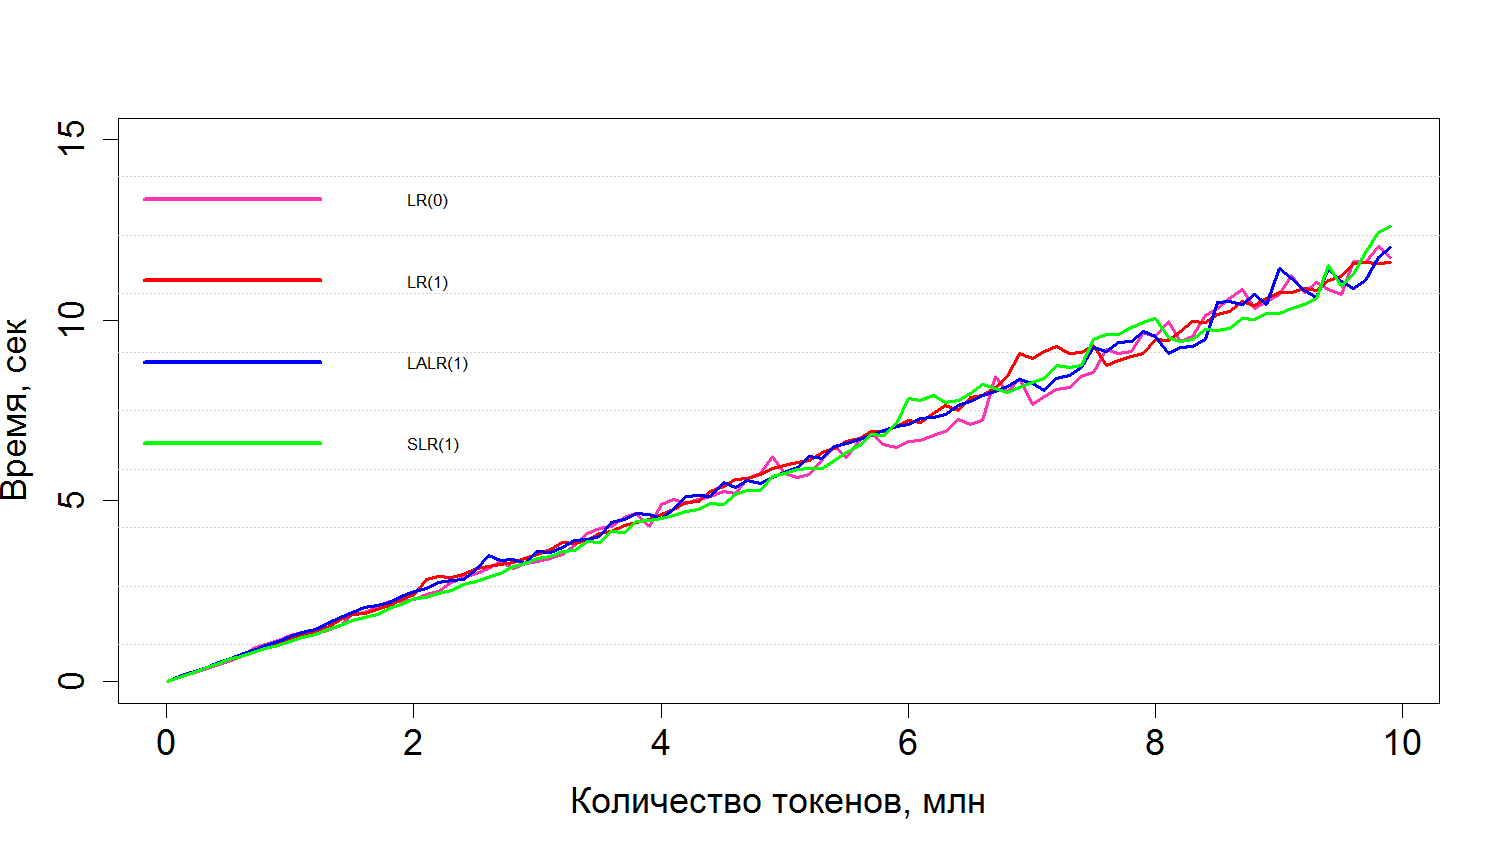
\includegraphics[width=1\textwidth]{EasyCalc/EasyCalc.png}}
  \caption{Время работы анализаторов для грамматики \textit{EasyCalc}}
  \label{EasyCalc}
  \centering
\end{figure}

\subsection{Эксперимент 2}
Рассмотроим более сложную грамматику \textit{Calc} калькулятора с выражениями (листинг~\ref{lst:Calc}).
\begin{listing}[H]
\begin{minted}
[
frame=lines,
framesep=2mm,
baselinestretch=1.2,
fontsize=\small
]
{fsharp}
[<Start>]
calc : statementList EOF { $1 }
statementList : statement SEP statementList { $1::$3 }
              | statement SEP { [$1] }
statement : expr { $1 }
          | ID EQ expr { $3 }
expr : multExpression PLUS multExpression { $1 + $3 }
     | multExpression MINUS multExpression { $1 - $3 }
     | multExpression { $1 }
atom : ID { $1 }
     | INT { $1 }
     | LBRACE expr RBRACE { $2 }
multExpression : atom MULT atom { $1 * $3 }
               | atom DIV atom { $1 / $3 }
               | atom { $1 }
\end{minted}
\caption{Грамматика \textit{Calc}}
\label{lst:Calc}
\end{listing}

Данная грамматика кроме бинарных операций позволяет записать ещё и выражения. Например:

\centerline{x=5;y=x*2;z=((17*x+36*y)+8);}


{\large \textbf{Результаты сравнения}}

Поскольку данная грамматика не является LR(0), но является SLR(1)-грамматикой, проведено сравнение на алгоритмах LR(1), SLR(1) и LALR(1).
На рис.~\ref{CalcLR1}, \ref{CalcSLR1}, \ref{CalcLALR1} изображена зависимость среднего времени работы синтаксического анализатора по 10-ти запускам от длины входной цепочки. Длина входной цепочки изменяется от 4 000 000 до 80 000 000 токенов.

\begin{figure}[h]
  \center{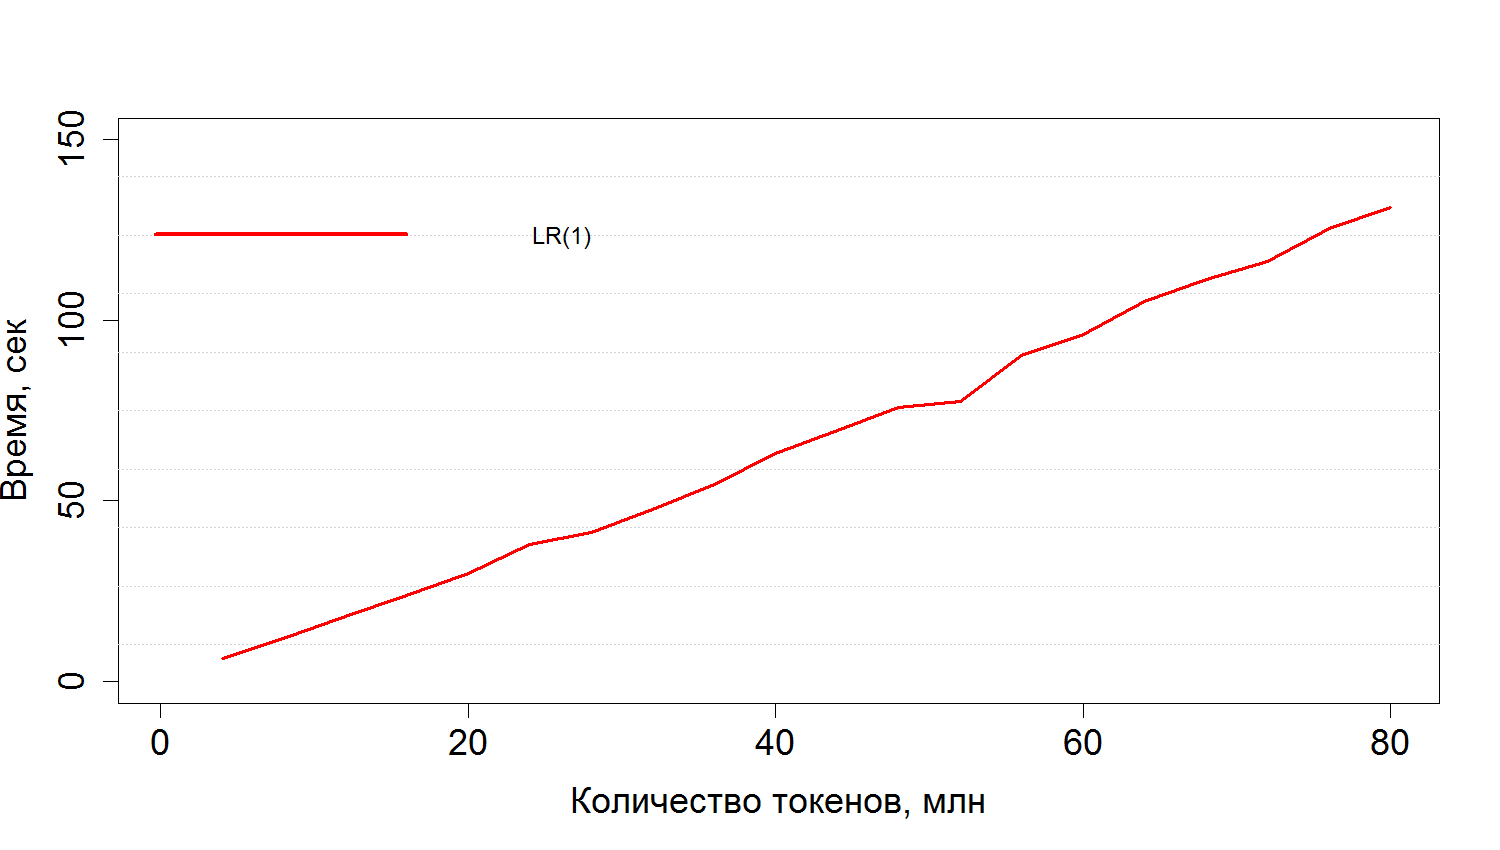
\includegraphics[width=1\textwidth]{Calc/LR1.png}}
  \caption{Время работы LR(1)-анализатора для грамматики \textit{Calc}}
  \label{CalcLR1}
  \centering
\end{figure}

\begin{figure}[H]
  \center{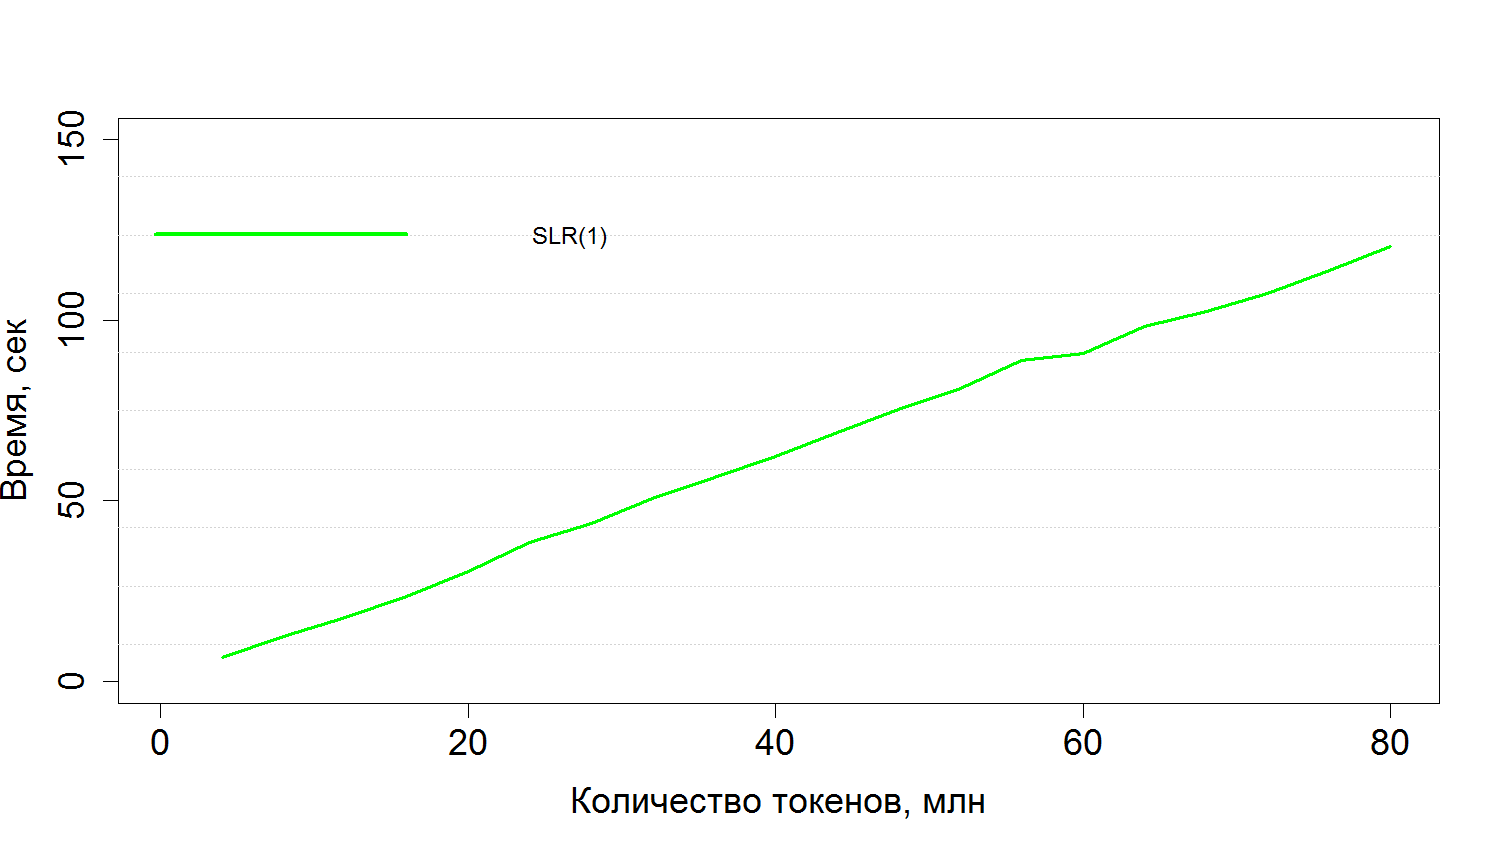
\includegraphics[width=1\textwidth]{Calc/SLR1.png}}
  \caption{Время работы SLR(1)-анализатора для грамматики \textit{Calc}}
  \label{CalcSLR1}
  \centering
\end{figure}

\begin{figure}[H]
  \center{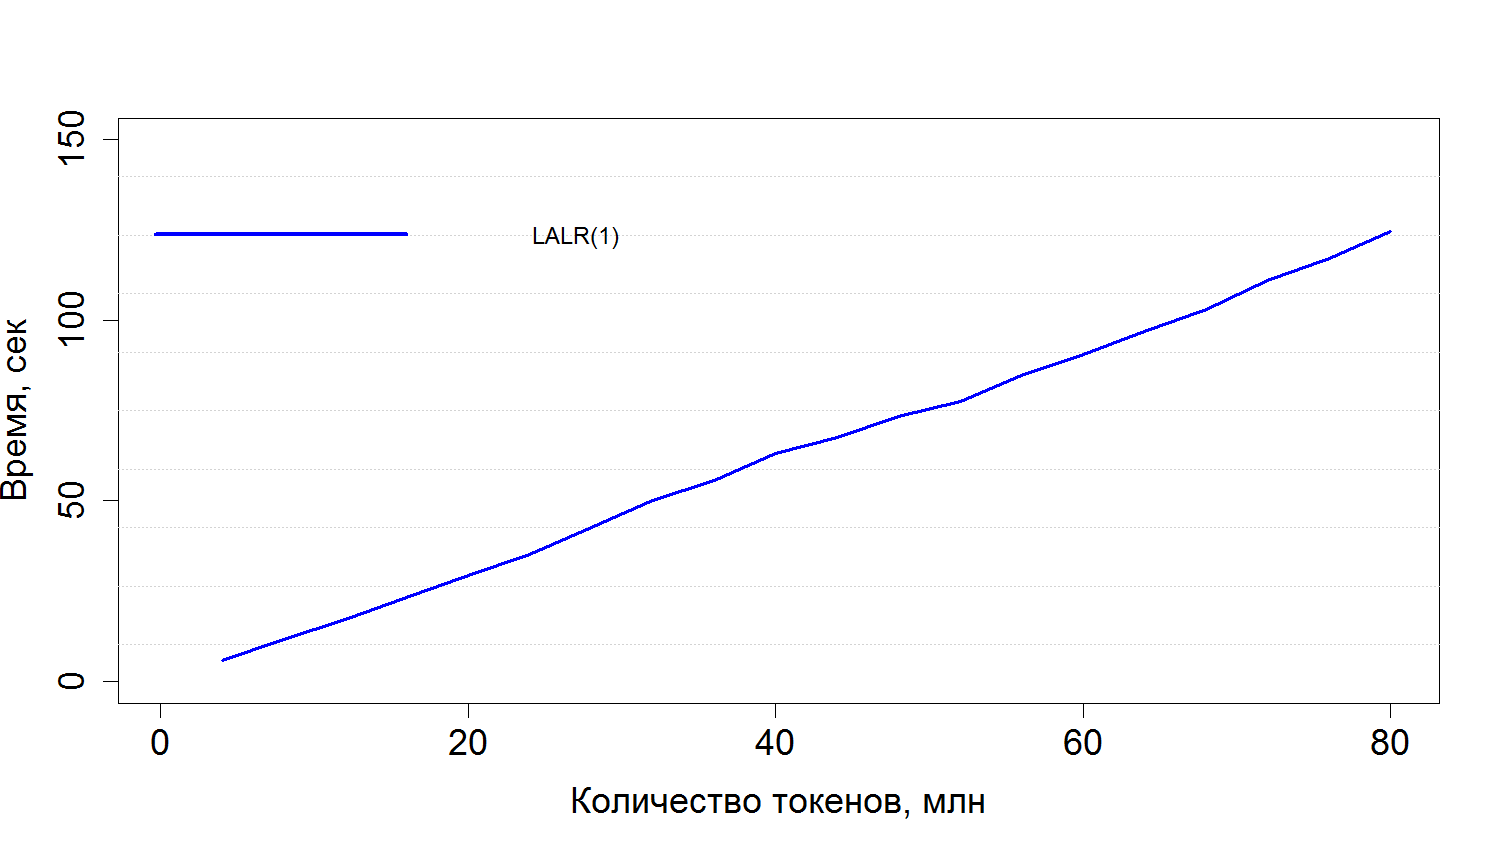
\includegraphics[width=1\textwidth]{Calc/LALR1.png}}
  \caption{Время работы LALR(1)-анализатора для грамматики \textit{Calc}}
  \label{CalcLALR1}
  \centering
\end{figure}

В табл.~\ref{tab:Calc} представлены некоторые результаты измерения среднего времени работы анализатора и среднеквадратического отклонения для грамматики \textit{Calc}.

\begin{table}[h]
\begin{center}
\begin{tabular}{|c|l|c|c|c|}
\hline  
 & Кол-во токенов & LR(1) & SLR(1) & LALR(1) \\ 
\hline  
 Среднее & 4 000 000 &  6.2 & 6.1 & 5.8 \\  
\cline{2-5}
время, & 15 000 000 & 24.1 & 23.5 & 22.3 \\  
\cline{2-5}
сек & 30 000 000 & 49.9 & 43.8 & 42.5 \\
\cline{2-5}
 & 55 000 000 & 87.7 & 81.6 & 84.6 \\
\cline{2-5}
 & 80 000 000 & 131.1 & 120.3 & 124.4 \\
\hline
\hline
Средне- & 4 000 000 & 0.197 & 0.108 & 0.037 \\  
\cline{2-5}
квадратич. & 15 000 000 & 0.201 & 0.13 & 0.076 \\  
\cline{2-5}
откл., & 30 000 000 & 0.328 & 0.462 & 0.421 \\
\cline{2-5}
сек & 55 000 000 & 0.463 & 0.901 & 0.363 \\
\cline{2-5}
 & 80 000 000 & 1.987 & 0.862 & 1.201 \\               
\hline  
\end{tabular}
\end{center}
\caption{\label{tab:Calc} Результаты замеров для грамматики \textit{Calc}}
\end{table}

На рис.~\ref{Calc} представлены результаты времени работы для выбранных алгоритмов.

\begin{figure}[h]
  \center{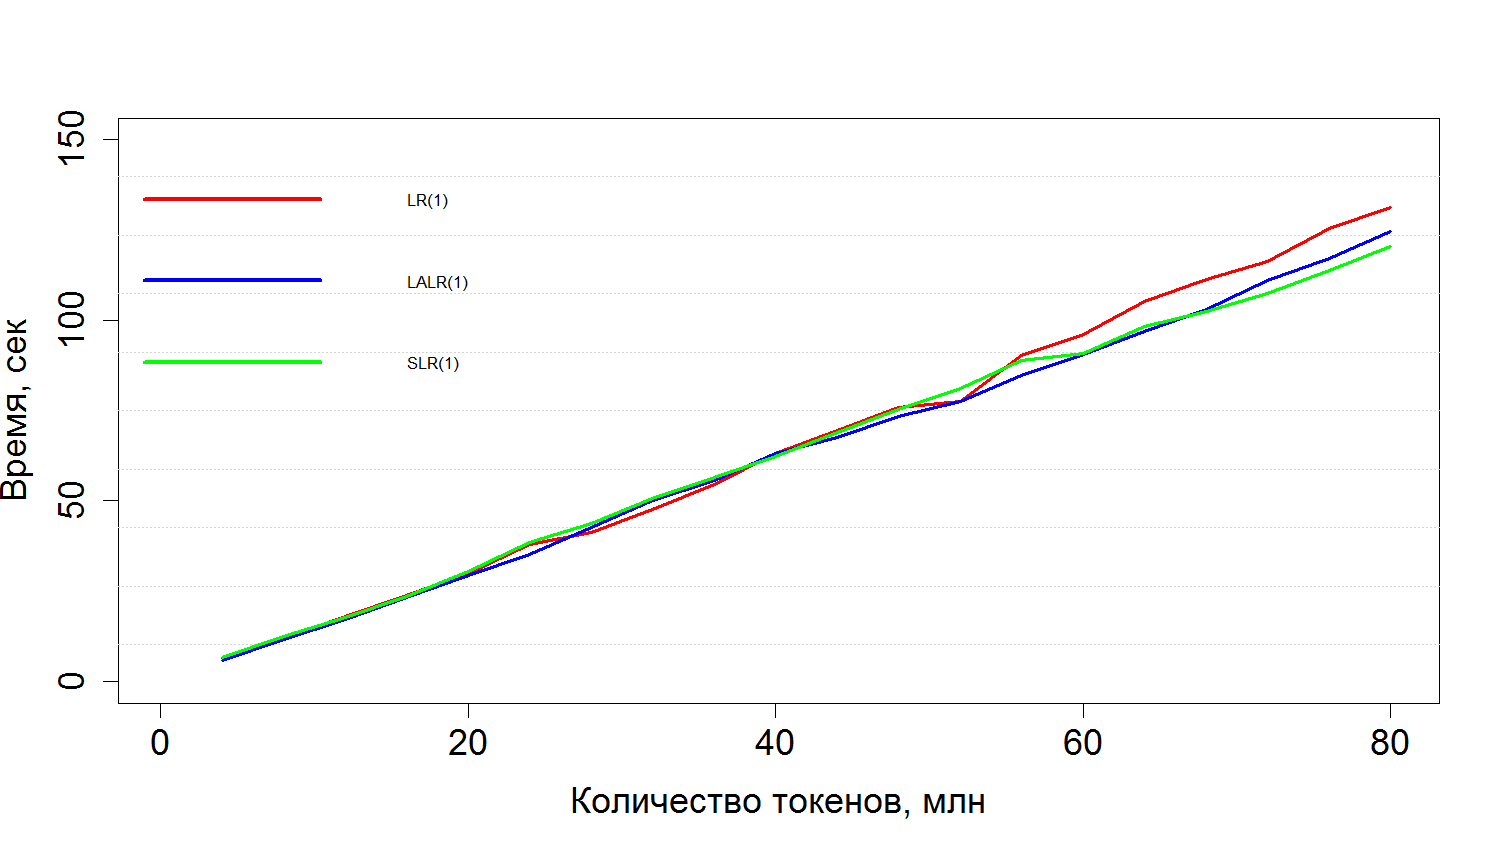
\includegraphics[width=1\textwidth]{Calc/Calc.png}}
  \caption{Время работы анализаторов для грамматики \textit{Calc}}
  \label{Calc}
  \centering
\end{figure}

\subsection{Вывод}

Полученная в результате интеграции платформа была протестирована на различных грамматиках и входах.

Проведено сравнение времени работы алгоритмов табличного восходящего синтаксического анализа на грамматиках \textit{EasyCalc} и \textit{Calc}. На больших входных данных, когда длина цепочки достигает порядка десятков миллионов токенов, начинает сказываться разница в размерах таблиц. Как известно, LR(1)-таблицы имеют больший размер.

В книге \cite{book:compilles} говорится о том, что LALR-таблица компактнее, то есть она занимает меньше памяти. Но стремление уменьшить количество потребляемой памяти было актуально раньше, когда у компьютеров было мало памяти.
Таким образом, современным компьютерам не важен размер таблиц.


%Возникает проблема: LR(0) ~--- самый узкий класс грамматик, то есть, если грамматика является LR(1), то не обязательно она будет LR(0).
%Сложной задачей является написание грамматик. Даже калькулятор не является LR(0)-грамматикой, но является LALR(1).

% У заключения нет номера главы
\section*{Заключение}
В ходе данной работы получены следующие результаты:
\begin{itemize}
\item
реализована интеграция YaccConstructor с инструментом Facio (F\#);
\item
проведено сравнение времени работы анализаторов, сгенерированных с использованием таких алгоритмов табличного восходящего синтаксического анализа, как LR(0), LR(1), LALR(1), SLR(1).
\end{itemize}

Исходный код можно посмотреть в репозитории проекта: \newline \href{https://github.com/YaccConstructor/YaccConstructor}{https://github.com/YaccConstructor/YaccConstructor}, автор — \textit{emavchun}.

Дальнейшим развитием данной работы может быть разработка отдельного приложения, которое на вход получает лексическую и синтаксическую спецификации языка, желаемый алгоритм восходящего анализа для генерации синтаксического анализатора и входную цепочку. Результатом работы данной программы являются графики зависимости времени, затраченного на синтаксический анализ, от длины входной цепочки. Также должна быть возможность отображения графиков для всех алгоритмов в одном окне для наглядного сравнения. Для построения графиков можно использовать библиотеку F# Charting \cite{link:fSharpCharting}.


\setmonofont[Mapping=tex-text]{CMU Typewriter Text}
\bibliographystyle{ugost2008ls}
\bibliography{diploma.bib}
\end{document}
